%%%%%%%%%%%%%%%%%%%%%%%%%%%%%%%%%%%%%%%%%
% Makoto Technical Report
% LaTeX Template
% Version 1.0 (December 6, 2024)
%
% This template originates from:
% https://www.LaTeXTemplates.com
%
% Author:
% Vel (vel@latextemplates.com)
%
% License:
% CC BY-NC-SA 4.0 (https://creativecommons.org/licenses/by-nc-sa/4.0/)
%
%!TEX program = xelatex
% Note: this template must be compiled with XeLaTeX rather than PDFLaTeX
% due to the custom fonts used. The line above should ensure this happens
% automatically, but if it doesn't, your LaTeX editor should have a simple toggle
% to switch to using XeLaTeX.
%
%%%%%%%%%%%%%%%%%%%%%%%%%%%%%%%%%%%%%%%%%

%----------------------------------------------------------------------------------------
%	CLASS, PACKAGES AND OTHER DOCUMENT CONFIGURATIONS
%----------------------------------------------------------------------------------------

\documentclass[
	a4paper, % Paper size, use either a4paper or letterpaper
	%unnumberedsections, % Uncomment for no section numbering
]{CSMakotoTechnicalReport}

\addbibresource{sample.bib} % BibLaTeX bibliography file

%----------------------------------------------------------------------------------------
%	REPORT INFORMATION
%----------------------------------------------------------------------------------------

\reporttitle{Aquí va el Título\\ titulooooo} % The report title to appear on the title page, include new lines if needed

\reportsubtitle{Aquí ingresa una frase\\ interesante que te guste} % Report subtitle, include new lines if needed

\reportauthors{Created by:\\\smallskip Diego Oxacopa (diegooxacopa64@gmail.com)} % Report authors/group/department, include new lines if needed

\reportdate{\today} % Report date, include new lines for additional information if needed

%------------ ENCABEZADO --------------------------------
%ENCABEZADO DEL DOCUMENTO
\leftheadercontent{Universidad Nacional de Moquegua} % Report title or other text to appear in the left header

%ENCABEZADO LOGO DEL DOCUMENTO
\rightheadercontent{
\includegraphics[width=3cm]{Images/unamlogo.jpeg}} % The content in the right header, you may want to add your own company logo or use your company/department name or leave this command empty for no right header content
%--------------------------------------------------------

%----------------------------------------------------------------------------------------

\begin{document}

%----------------------------------------------------------------------------------------
%	TITLE SECTION
%----------------------------------------------------------------------------------------

% The code here uses the information set in the REPORT INFORMATION block above and does not need to be modified unless you want to change the layout of the title section.

\thispagestyle{empty} % Suppress headers and footers on this page

\vspace*{-0.075\textheight} % Pull logo into top margin

% LOGO EN PAGINA TITULO
\hfill
\includegraphics[width=5cm]{Images/unamlogo.jpeg} % Right-aligned company logo

\vspace{0.06\textheight} % Vertical whitespace

{\large\raggedright\reportdate\par} % Report date

\vspace{0.01\textheight} % Vertical whitespace

{\fontsize{32pt}{34pt}\selectfont\raggedright\textbf{\reporttitle}\par} % Report title

\vspace{0.03\textheight} % Vertical whitespace

{\Large\raggedright\textit{\textbf{\reportsubtitle}}\par} % Subtitle

\vspace{0.06\textheight} % Vertical whitespace

{\large\raggedright\reportauthors\par} % Report authors, group or department

\vspace{0.12\textheight} % Vertical whitespace

%----------------------------------------------------------------------------------------

\begin{multicols}{2} % Begin two column mode

%----------------------------------------------------------------------------------------
%	TABLE OF CONTENTS
%----------------------------------------------------------------------------------------

\tableofcontents % Output the table of contents, automatically generated from the section commands used in the document

%----------------------------------------------------------------------------------------
%	SECTIONS AND PARAGRAPHS
%----------------------------------------------------------------------------------------





%----------------------------------------------------------------------------------------
%	VIEW OF SAMPLES FOR 
%----------------------------------------------------------------------------------------
\begin{figure}[H]
	\centering
	
\includegraphics[width=\linewidth]{samples/image.png}
\end{figure}

\begin{quote}
	\textbf{\LARGE ``}Lorem ipsum dolor sit amet, consectetur adipiscing elit. Praesent porttitor arcu luctus, imperdiet urna iaculis, mattis eros. Pellentesque iaculis odio vel nisl ullamcorper, nec faucibus ipsum molestie. Sed dictum nisl non aliquet porttitor. Etiam vulputate arcu dignissim, finibus sem et, viverra nisl. Aenean luctus congue massa, ut laoreet metus ornare in.\textbf{''}
	
	\hfill--- John Smith, 1972
\end{quote}



\begin{figure}[H]
	\centering
	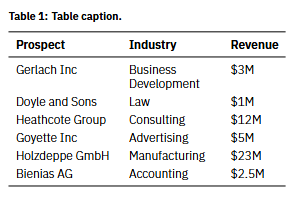
\includegraphics[width=\linewidth]{samples/image2.png}
\end{figure}


\begin{table}[H] % [H] forces the table to be output where it is defined in the code (it suppresses floating)
	\caption{Table caption.}
	\begin{tabular}{L{0.35\linewidth} L{0.31\linewidth} L{0.17\linewidth}} % Table column widths and alignment (L, C or R)
		\toprule
		\textbf{Prospect} & \textbf{Industry} & \textbf{Revenue} \\
		\midrule
		Gerlach Inc & Business Development & \$3M\\
		Doyle and Sons & Law & \$1M\\
		Heathcote Group & Consulting & \$12M\\
		Goyette Inc & Advertising & \$5M\\
		Holzdeppe GmbH & Manufacturing & \$23M\\
		Bienias AG & Accounting & \$2.5M\\
		\bottomrule
	\end{tabular}
	\label{tab:example}
\end{table}


\begin{figure}[H]
	\centering
	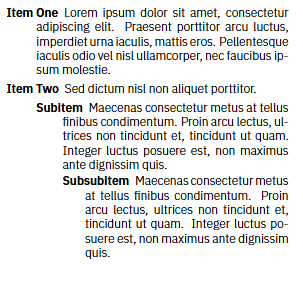
\includegraphics[width=\linewidth]{samples/image3.png}
\end{figure}


\begin{description}
	\item[Item One] Lorem ipsum dolor sit amet, consectetur adipiscing elit. Praesent porttitor arcu luctus, imperdiet urna iaculis, mattis eros. Pellentesque iaculis odio vel nisl ullamcorper, nec faucibus ipsum molestie. 
	\item[Item Two] Sed dictum nisl non aliquet porttitor.
	\begin{description}
		\item[Subitem] Maecenas consectetur metus at tellus finibus condimentum. Proin arcu lectus, ultrices non tincidunt et, tincidunt ut quam. Integer luctus posuere est, non maximus ante dignissim quis.
		\begin{description}
			\item[Subsubitem] Maecenas consectetur metus at tellus finibus condimentum. Proin arcu lectus, ultrices non tincidunt et, tincidunt ut quam. Integer luctus posuere est, non maximus ante dignissim quis.
	\end{description}
	\end{description}
	\item[Item Three] Etiam vulputate arcu dignissim, finibus sem et, viverra nisl. Aenean luctus congue massa, ut laoreet metus ornare in. Nunc fermentum nisi imperdiet lectus tincidunt vestibulum at ac elit. Nulla mattis nisl eu malesuada suscipit.
\end{description}


\begin{figure}[H]
	\centering
	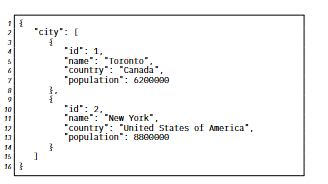
\includegraphics[width=\linewidth]{samples/image4.png}
\end{figure}

\begin{lstlisting}
{
	"city": [
		{
			"id": 1,
			"name": "Toronto",
			"country": "Canada",
			"population": 6200000
		},
		{
			"id": 2,
			"name": "New York",
			"country": "United States of America",
			"population": 8800000
		}
	]
}
\end{lstlisting}



\end{multicols}
\end{document}
